\documentclass[12pt,a4paper]{article}

\usepackage{color}
\usepackage{amsxtra}  
\usepackage{amsthm}
\usepackage{amssymb}
\usepackage{amsfonts}
\usepackage{graphicx}  
\usepackage{rotating}


\begin{document}

\title{Report: Modeling Chromosomes During Meiosis in Fission Yeast}
\author{Wenwen Huang}
\date{\today}

\maketitle

\section{Introduction}
\label{sec:introduction}

During meiosis I in Fission Yeast (S. pombe), a dramatic chromosome movement
named nuclear oscillation is observed. Spindle Pole Body (SPB), which is a
centrosome like organelle embedded in the nucleus membrane and bonded to the
Microtubes out of nucleus, drives the nucleus moves forward and backward in the
cylinder shaped cell. Chromosomes in the nucleus, which are of course moving
together, are arranged and recombined during this period. 

Nuclear oscillation is believed to play an important role for chromosome
paring and recombination, which are crucial for the following separating
procedure. The exact process how these movements facilitate or suppress
paring and recombination is not clearly understood. Here, we propose an
realistic physical model and try to describe the chromosome movements during
nuclear oscillation quantitatively, aiming to understand the biological
functionalities of these chromosome movements.


\section{Chromosome modeled by polymer}
\label{sec:chromosome}

During nuclear oscillation, chromosomes are compacted and sister chromatins are
adhered together form a much thicker rod like structure comparing to single DNA
strand. Moreover, both ends of the chromosomes are bonded to the SPB. Thus the
topology of chromosomes is ring like structure. 
\begin{figure}[htpb]
	\centering
	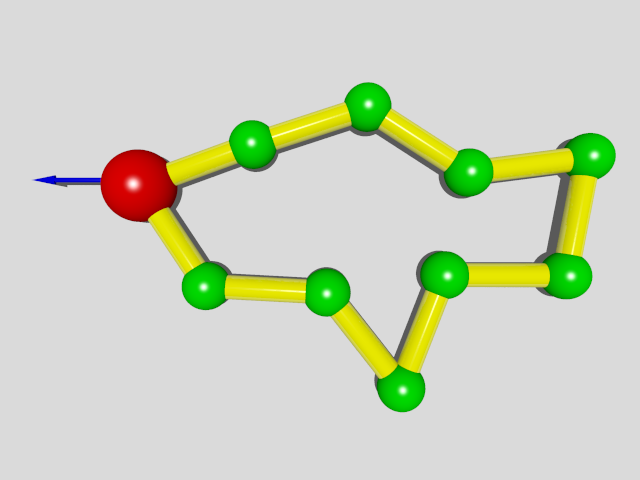
\includegraphics[width=0.8\linewidth]{figs/Ring0.png}
	\caption{A sketch for bead-rod model representing one chromosome, red
		bead represents SPB.}
	\label{fig:Ring0}
\end{figure}

Chromosomes in the nucleus during nuclear oscillation are modeled by polymers.
More specifically, the model that bead connected by massless rod is employed.
A sketch is shown in figure~\ref{fig:Ring0}. The red bead representing SPB is
driven by a force and other beads are connected through rigid rod, which means
the length of each rod is unchangeable.   

\begin{figure}[htpb]
	\centering
	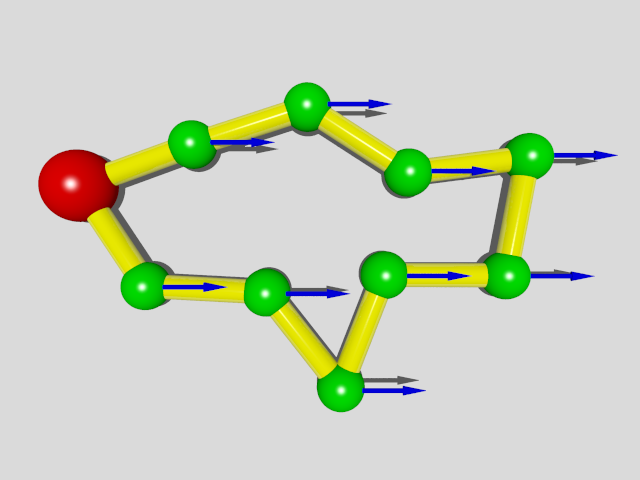
\includegraphics[width=0.8\linewidth]{figs/Ring1.png}
	\caption{Sketch of pinned bead-rod ring in co-moving frame.}
	\label{fig:Ring1}
\end{figure}
It would be a good approximation that the SPB is driven by a periodic force
during nuclear oscillation. However, we start from the simplest scenario that
the driven force is constant. Experimentally, it is shown that the speed
of SPB is almost constant when moving in one direction~\cite{Vogel2009}. So it
is nontrivial to consider the constant driven force case. In this case, we can
change to a co-moving frame, i.e., sitting on the SPB, then it is equivalent
to the scenario that SPB is pinned, and a constant force is imposed on all
other beads. See in another sketch figure~\ref{fig:Ring1}. 

Let us consider pinned polymer ring in external force field described above.
Denote the position of every bead using $\mathbf{r}_i$ where $i = 0,1,\cdots N$.

\section{Simulation}
\label{sec:simulation}

\subsection{Monte Carlo Simulation}
\label{sub:monte_carlo_simulation}

\subsection{Brownian Dynamics Simulation}
\label{sub:brownian_dynamics_simulation}

\section{Theory}
\label{sec:theory}

The square mean position of every bead writes
\begin{equation}
	\left<\mathbf{r}_i\right>^2  = 
T^{2} \left(\log{\left (\frac{\mu}{T \sinh{\left (\frac{\mu}{T} \right )}} \right )} - \log{\left (\frac{i - \mu}{T \sinh{\left (\frac{1}{T} \left(i - \mu\right) \right )}} \right )}\right)^{2}
\end{equation}
where $T$ is the dimensionless temperature and $\mu$ is chemical potential, i.e.
$\mu = (N+1)/2$ in our case.

\section{Outlook}
\label{sec:outlook}


\bibliography{report}
\bibliographystyle{plain}

\end{document}
